\problemname{Interception}

\illustration{0.4}{canned-phone}{\href{https://pixabay.com/en/canned-phone-box-cable-funny-fun-568057/}{Photo} by Michael Schwarzenberger, public domain}%
\noindent
You are helping your local Neighborhood Surveillance Association 
setting up a surveillance system on your street in order to identify
the culprits behind some recent unfortunate dog doo incidents.

The system in question consists of listening devices placed on the
tin-can phone lines of the street (the idea being that sooner or later
the dog doo malefactors will mess up and discuss their dirty deeds
over the phone).  Each listening device is placed on one of the phone
lines connecting the houses, and will intercept all calls that are routed
along that phone line.

The phone line network looks as follows.  One side of the street has
odd-numbered houses, and the other side has even-numbered houses.  The
numbers are lined up so that odd-numbered house $i$ is directly across
the street from even-numbered house $i+1$.  On both sides of the
street, there are direct phone lines between adjacent pairs of houses.
In addition there are two direct phone lines connecting the two sides
of the street.  Both of these two phone lines connect a house with
the house directly across from it.

Calls between two houses on the same side of the street are routed
along the direct path between the two houses, without going to the
other side of the street.  For calls between two houses on opposite
sides of the street, we have information about which of the two direct
connections across the street the call will use.

From previous ventures, we do know which people on the street are on
speaking terms with each other.  We would like to place listening
devices in such a way that we can intercept all phone calls.  In other
words, for every pair of people that are on speaking terms with each
other, there must be a listening device on the route between their houses.

Your job is to find a way to do this using the minimum possible number
of listening devices (since they are kind of expensive and we burnt
most of our budget on the barbecue last week).

\begin{figure}[!h]
  \centering
  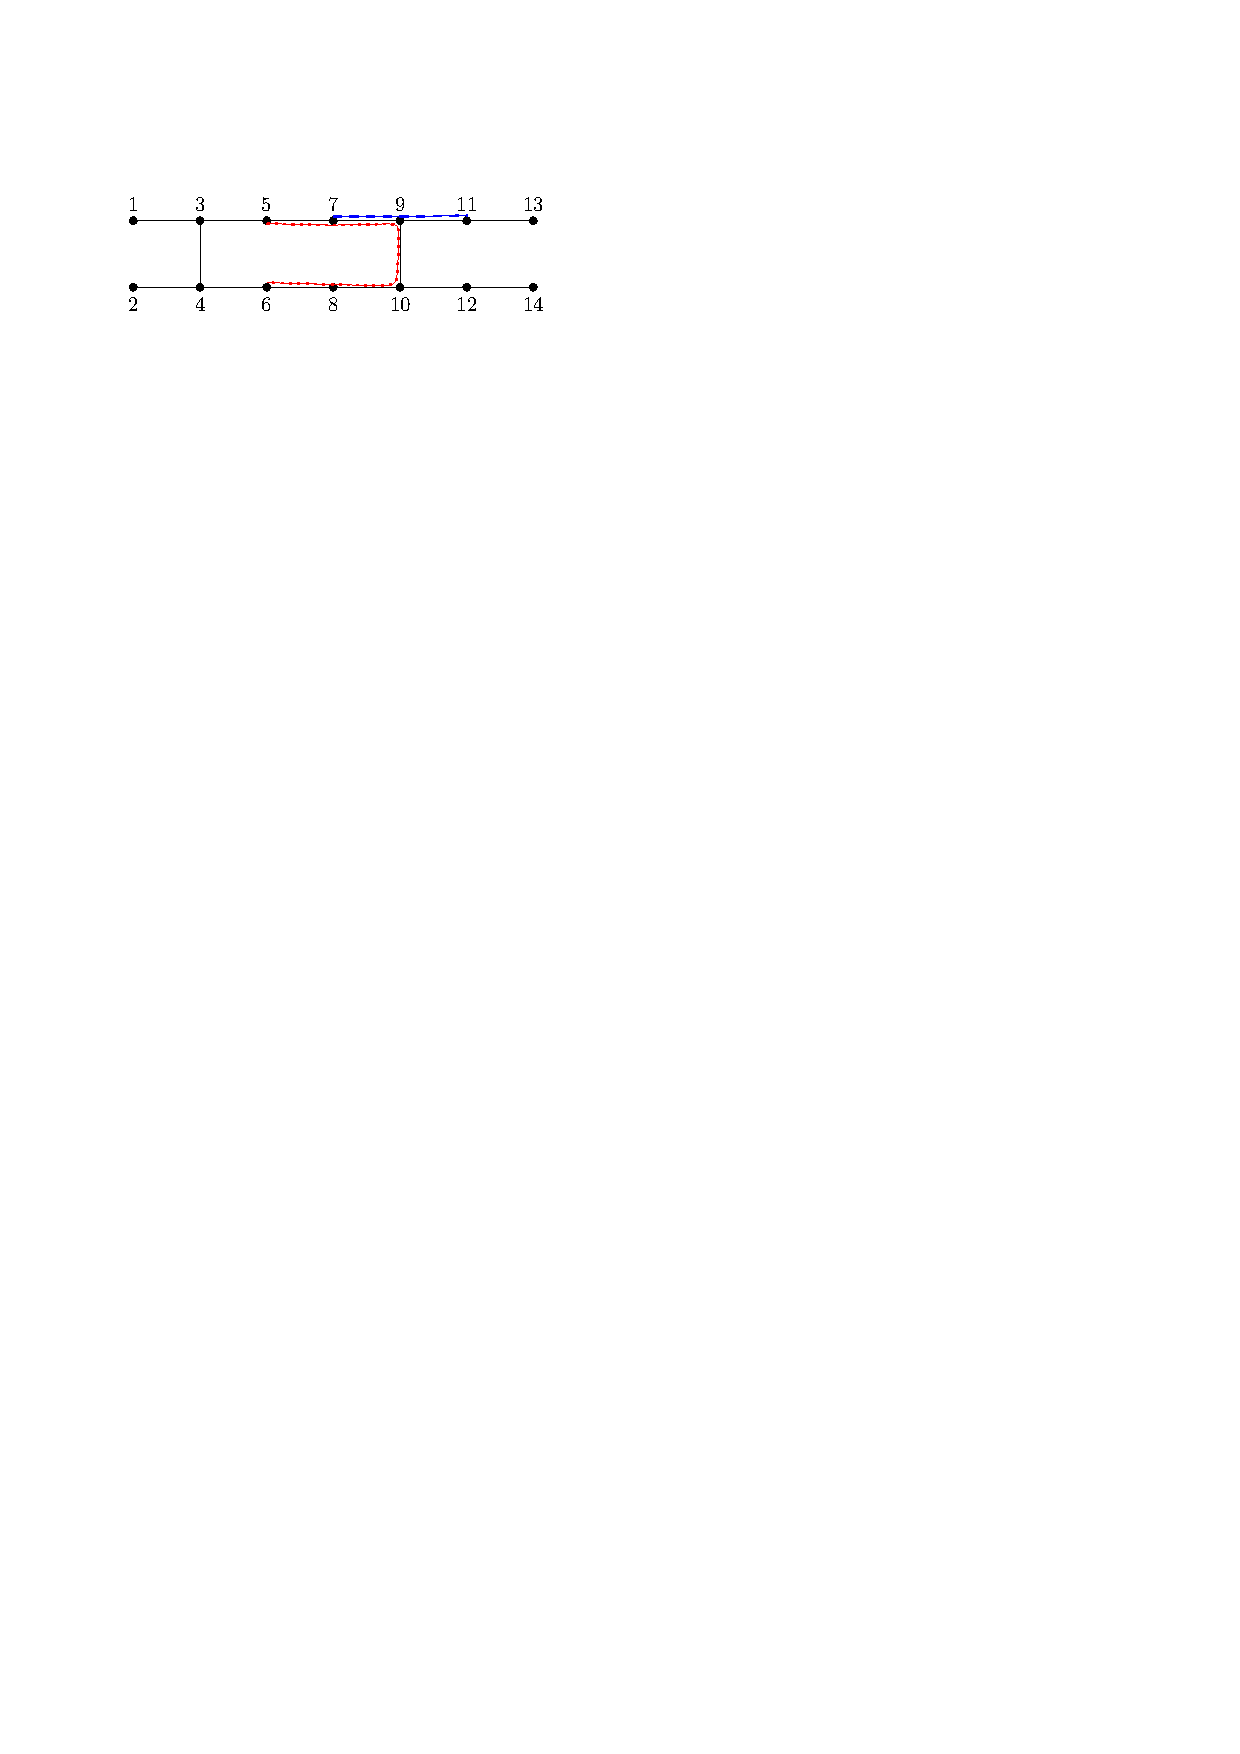
\includegraphics[width=0.6\textwidth]{sample}
  \caption{Illustration of the phone line network in Sample Input 1.
    There are $14$ houses, $7$ on each side, and the two direct
    connections across the street connect house $3$ with house $4$,
    and house $9$ with house $10$.  The people in houses $7$ and $11$
    are on speaking terms, and calls between them are routed via house
    $9$.  The people in houses $5$ and $6$ are also on speaking terms,
    and calls between them are routed via houses $7$, $9$, $10$, and
    $8$.  Sample Input 2 is similar, but there the calls between $5$
    and $6$ are instead routed via the direct connection between
    houses $3$ and $4$.}
 \label{fig:surveillance sample}
\end{figure}

\section*{Input}

The first line of input consists of four integers $n$, $m$, $c_1$, and
$c_2$ ($4 \le n \le 250\,000$, $1 \le m \le 500\,000$, $1 \le c_1
< c_2 < n$), where $n$ is even and denotes the number of houses
on the street, $m$ is the number of pairs of people that are on
speaking terms with each other, and finally $c_1$ and $c_2$ are odd,
denoting that the two wires crossing the street go between houses
$c_1$ and $c_1+1$, and between houses $c_2$ and $c_2+1$.

Then follow $m$ lines, each beginning with two distinct integers $a$
and $b$ between $1$ and $n$ (inclusive), indicating that the person in
house $a$ is on speaking terms with the person in house $b$.  If the
houses are on opposite sides of the street, they are followed by an
integer $c \in \{c_1, c_2\}$ indicating that calls between $a$ and $b$
are routed along the direct connection between $c$ and $c+1$.  Each
pair $\{a,b\}$ appears at most once in the input.

\section*{Output}

Output one line with an integer $\ell$, the smallest possible number
of listening devices needed.  Then output $\ell$ lines, each
containing a pair of integers, describing between which pairs of
houses listening devices should be placed (of course, each of these
pairs must be directly connected by a phone line).  If there is more
than one optimal solution, you may output any one of them.
